\FloatBarrier
\subsection{Newtonian noise}
\label{NewtonianNoise}
A source of noise within the gravitational wave detector that originates from
the local seismic activity is GGN (gravity gradient noise), also referred to as NN
(Newtonian noise). The seismic activity causes perturbations in the local
gravity field, which couples directly to the interferometer test masses. Up
until now, no experimental methods for NN suppression exist and suppressing
this noise source is difficult. As such, it is crucial to identify sites that
exhibit low seismicity. It is expected that an underground environment is to
improve on all associated sources of seismic noise spectral amplitude,
including seismically induced NN. Furthermore, the local environmental
conditions underground are usually stable (and controllable) and
anthropogenic-induced seismicity is much more controllable underground, where
access is limited. The following subsections discuss this issue.

In Subsection~\ref{subsub:NNanalyticalestimation} a simple analytical
estimations of NN is discussed. The power spectrum of NN is written as a
function of a measurable seismic quantity, under the hypothesis of homogeneity
for the medium, and neglecting any kind of effects from underground
structures.  This kind of approach is possible only with simplified models,
however it can provide guidelines expecially when detailed informations about
the geological structure of the site are not available.

A complimentary approach to analytical estimation, based on finite element
models, is presented is Subsection~\ref{subsub:NNfiniteelementmodels}. This is
the natural way to give a refined evaluation of aspects that cannot be
considered easily in the analytical approach, such as the effect of the
infrastructures and of the geological details, for example inhomogeneities.

Finally, two NN subtraction schemes are presented. In Subsection~\ref{subsub:AmbientNNsubtraction} a subtraction scheme is presented to monitor the NN induced by the ambient seismic background, using a seismic sensor array. This is the approach that must be used when it is not possible to recognise a dominant and localised source of seismic noise.

On the other hand if a strong and coherent source of noise is known (for example a pump), a single accelerometer can be used to monitor the induced seismic field. Using optimal filtering, the NN transfer function is estimated from the source to the interferometer test mass, and can be subtracted from the data. Details about this subtraction procedure are presented in Subsection~\ref{subsub:NNsubtractionperiodic}.

\FloatBarrier
\subsubsection{A simplified NN estimate}
\label{subsub:NNanalyticalestimation}
For a given distribution of masses, which can be described by a mass density function $\rho({\bf x},t)$, the acceleration experienced by a test mass located at ${\bf y}$ can be written as
\begin{eqnarray}
	{\bf a}^{NN}({\bf y},t)=G\int_{V}\rho({\bf x},t)
        \frac{\bf x-y}{|{\bf x-y}|^{3}}                        
        dV_{x}
	\label{eq3.1}
\end{eqnarray}
where the integration is extended to the volume $V$ of interest.

We are interested in the fluctuating part of this quantity when the medium is an elastic solid. From the expression of mass conservation we get
\begin{eqnarray}
	\dot{\rho}+{\boldsymbol \nabla}\cdot{\bf J}_{m}=0
	\label{eq3.3}
\end{eqnarray}
where the mass density current is given by ${\bf J}_{m}=\rho_{0}({\bf x})\dot{\boldsymbol \xi}({\bf x},t)$, $\rho_{0}$ being the density of the medium in the static configuration and ${\boldsymbol \xi}$ its small displacement at a given point.

By inserting Eq.~(\ref{eq3.3}) inside Eq.~(\ref{eq3.1}) we find
\begin{eqnarray}
	{\bf a}^{NN}({\bf y},\omega)=G\int_{V} {\boldsymbol \nabla} \cdot [\rho_{0}({\bf
	x}){\boldsymbol \xi}({\bf x},\omega)]
        \frac{\bf x-y}{|{\bf x-y}|^{3}}                        
        dV_{x} \label{eq3.4}
\end{eqnarray}
Note that this expression contains two different effects, as can be seen
expanding the derivative. The term proportional to $\rho_{0}
{\boldsymbol \nabla}\cdot {\boldsymbol \xi} $ describes the fluctuations of
the local density connected to the compression of the medium, while
${\boldsymbol \xi} \cdot {\boldsymbol \nabla}\rho_{0}$ takes into account
the effect of the movement of density inhomogeneities, for example at the
surface boundary.

Starting from Eq.~(\ref{eq3.4}) a general theory about the connection between seismic measurements and NN can be developed. We will not give here the details, which can be found for example in~\cite{Beker2010GRG}. The general idea is to decompose seismic motion in normal modes, which are supposed to behave as oscillators coupled to unknown stochastic forces. By measuring quantities connected to seismic fluctuations (for example the power spectrum of horizontal and/or vertical displacement, or the correlation between displacements at two different points) we can get information about the excitation of these oscillators. Using Eq.~(\ref{eq3.4}) these can be converted to an estimate of NN.

By making some additional assumptions a simple estimate of strain equivalent power spectrum of NN $S_{h}^{NN}$ can be done. We will present and discuss now this simplified result.

We model the ground as a homogeneous medium of given density $\rho_{0}$ and the longitudinal and transverse speeds of sound $c_{L}$, and $c_{T}$ respectively. The mirrors of the interferometer are supposed to be underground, inside a cavity whose effect can be seen to be not important in the low frequency regime we are interested to.

As we said there will be two kind of contributions, connected to surface and bulk fluctuations. The main assumption of the model is that the fluctuations associated to surface Raileigh waves are dominant. In this case both the contributions are exponentially damped with the depth, over a typical scale of $\ell \sim v_s (2\pi f)^{-1}$ where $v_s$ is the speed of sound and $f$ the frequency.

\begin{figure}[t!]
	\begin{center} 
		\includegraphics[width=16cm]{./Sec_SiteInfra/Figures/GeometricFactor.pdf} 
		\caption{The geometrical suppression factor $\mathcal{F}$ as a function of the ratio between the mode's wavelength and the length L of the interferometer arm. $\mathcal{F}$ suppresses the NN at low frequencies. It is normalized to one in the high frequency region, where the contribution of the motion of each test mass is uncorrelated and adds in quadrature.} 
		 \label{fig3.7} 
	\end{center}
\end{figure}


If we assume further that damping effects are negligible, so that each mode is excited essentially only at its natural frequency we can write now the final expression for the NN estimate as
\begin{eqnarray}
	\sqrt{\frac{S^{NN}_{h}(\omega)}{C^{seism}_{vv}(0;\omega)}}= \frac{4\pi G\rho_{0}}{L\omega^{2}\sqrt{2}} \times\bigg{(}\frac{2(\beta^{2}_{T}+1)e^{\beta_{L}Kz}-(1+2\beta_{L}+\beta^{2}_{T}) e^{Kz}}{\beta_{L}(\beta^{2}_{T}-1)}\bigg{)}\mathcal{F}\bigg{(}\frac{\omega L}{c_{T}\sqrt{x}}\bigg{)}^{1/2}
	\label{eq3.36}
\end{eqnarray}
where we choose to normalise the noise to the power spectrum of vertical surface seismic motion, $C^{seism}_{vv}(0;\omega)$. The function
\begin{eqnarray}
	\mathcal{F}(kL)=1+2J_{2}(kL)-\frac{2}{kL}J_{1}(kL)-\frac{1}{2}J_{2}(kL\sqrt{2})
	\label{eq3.33}
\end{eqnarray}
which appears in Eq.~(\ref{eq3.36}) describes the coherence between the gravitational accelerations of different test masses. It is apparently real and it goes to zero in the low frequency regime. This is due to the fact that when the wavelength of seismic modes is large compared with the interferometer size each mirror feels the same acceleration, so that the length of the resonant cavities in the arms of the interferometer does not fluctuate. Practically it can be set to one in the frequency range of interest.

Setting $z=0$ in Eq.~(\ref{eq3.36}) we can directly compare with previous estimates of NN on the surface~\cite{GGSaulson, GGCellaCuoco, GGThorne}, finding essentially an agreement.

The attenuation factor, which is the ratio between the NN amplitude at a depth $z$ and the one on the surface, can be obtained by the middle term in brackets in Eq.~(\ref{eq3.36}). It is plotted in Fig.~\ref{fig3.8} (left) for several selected frequencies, as a function of the depth.
\begin{figure}[t]
	\begin{center} 
		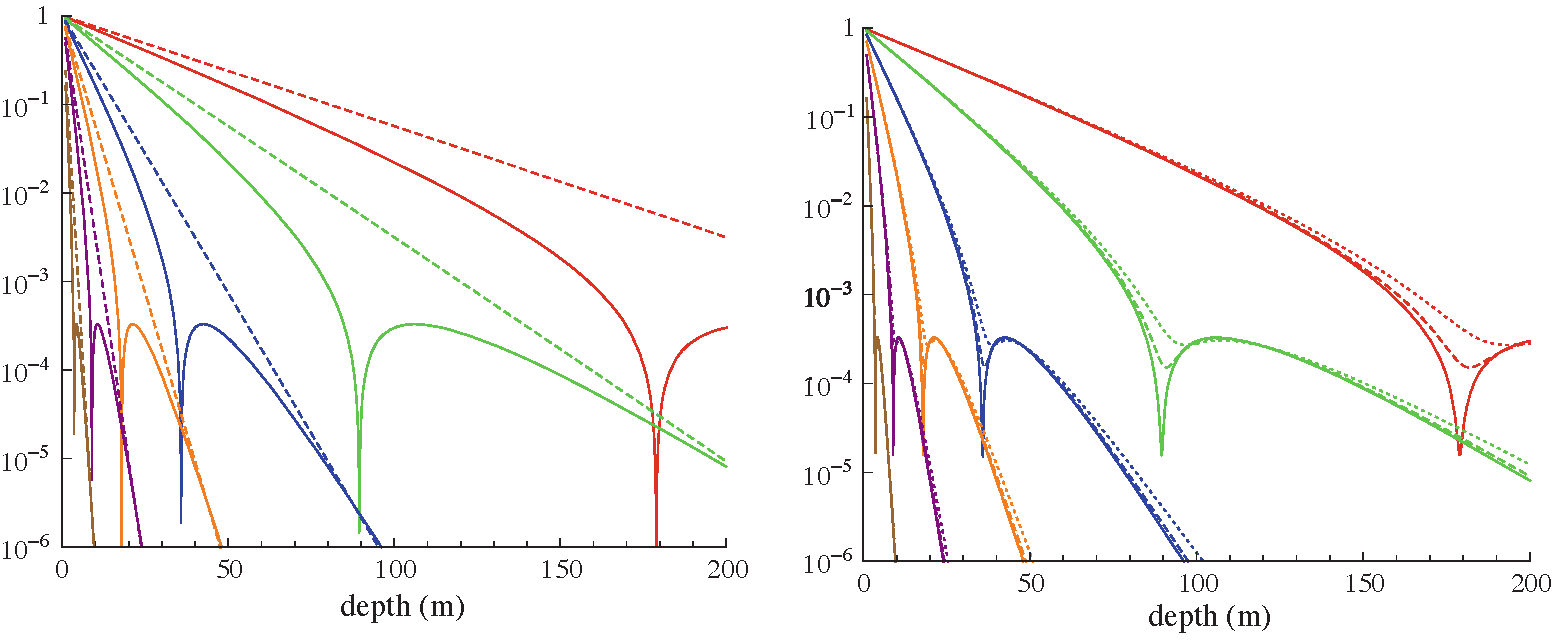
\includegraphics[width=16.5cm]{./Sec_SiteInfra/Figures/CellaNNTF.pdf} 
		\caption{{\em Left}. The Newtonian noise attenuation factor (vertical axis) predicted by Eq. (\ref{eq3.33}) as a function of depth (horizontal axis) for selected frequencies. The correspondence is red 1Hz, green 2Hz, blue 5Hz, orange 10Hz, purple 20Hz, and brown 50Hz. Here $c_{T}=220m/s$ and $c_{L}=440m/s$ (continuous curve) or $c_{L}=880m/s$ (dashed curve). The zero appears when the two exponentially damped factors in Eq. (\ref{eq3.33}) cancel. Before and after this point the decrease will be dominated by one of the two, therefore the decay constant changes. {\em Right}. The effect of the soil quality factor (vertical axis) as a function of depth (horizontal axis, in m) for selected frequencies. The quality factor is modeled using Eq. (\ref{eq3.36}) and corresponds roughly to $Q=10^{4}$ (continuous curve), $Q=10^{3}$ (dashed curve), and $Q=2\times10^{3}$ (dotted curve)}.  
		\label{fig3.8} 
	\end{center}
\end{figure}

Looking at Fig.~\ref{fig3.8}(left), at a given depth and frequency, the NN
contribution can be zero. This in a sense is an artifact of our oversimplified
model, and stems from our assumption that a mode contributes to the NN noise
only at its resonant frequency. Another consequence of this assumption is that
the vertical seismic correlation is proportional to $J_{0}\Big{(}\frac{\omega
r}{c_{T}\sqrt{x}}\Big{)}$, causing it to decrease quite slowly (as $r^{-1/2}$)
at large distances, which is unrealistic. We can take into account coherence
effects by add some damping to the seismic modes considered in the model. This
is equivalent to give a finite width to its resonant response. Just for
illustrative purpose we can choose a Gaussian line shape parameterized by a
width parameter $\Gamma$ and compare the result for the NN estimate. We do not
report the analytical details here, instead we present the result comparing
the attenuation factor at different values of $\Gamma$ in Fig.~\ref{fig3.8}
(right).

We see the expected smoothing effect, and also an apparent saturation of the
attenuation factor for the smallest soil quality factor $Q$. This is expected
since the soil quality factor is small corresponding to longer wavelength
modes, which are excited for a given frequency. The combination of the soil
quality factor and coherence effects have also impacts on the estimate of NN,
which will not be discussed here.

\FloatBarrier
\subsubsection{Finite element models}
\label{subsub:NNfiniteelementmodels}
Complimentary to the presented analytical descriptions of seismic activity, it will be come important, whenever considering a non-homogeneous medium or complex geologies, to have an accurate description of the seismic wave field. Simulations of such systems were accomplished using the FE (Finite Element) software package \textit{Comsol}~\cite{comsol}. In the FE framework 3D continuum is subdivided into small hexahedral elements. Within each element the relevant physical parameters, like displacement and stress, are approximated by spline functions of arbitrary order. The following section shows how the FE software can be used to predict the NN contributions from surface and bulk waves in homogeneous media. The analysis provides the basis for simulation in non-homogeneous and/or stratified soils.

The displacement wave field that results from a seismic disturbance, is governed by the elasto-dynamic equations. The wave field in a homogeneous elastic medium can be expressed as a combination of plane body waves~\cite{seismic_schevenels}. Two types of body waves exist, pressure (P) and shear (S) waves~\cite{seismic_achenbach}. In the case of P-waves the movement of a ground particles is parallel to the direction of wave propagation. For S-waves the particle motion is perpendicular to the direction of the wave. The characteristics of seismic waves can be described by the ground properties, parametrized by  the Young's modulus, $E$,  the density, $\rho$, and  the Poisson ratio, $\nu$, describing the relationship between shear and strain forces. The wave velocities are then given by
\begin{eqnarray}
	c_P = \sqrt{\frac{E(1-\nu)}{(1-2\nu)(1+\nu)\rho}},\mbox{ and} \hspace{0.5cm} c_S = \sqrt{\frac{E}{2(1+\nu)\rho}},
	\label{eq3.38}
\end{eqnarray}
for P and S-waves respectively. Typical values for hard-rock range from 3 - 6 km/s for $c_P$, and 1.5 - 4 km/s for $c_S$. In a medium that is bounded by another medium, such as air, or is composed of layers, surface and Head waves also exist. Head waves emerge in stratified media where modes propagating along an interface, cause energy to radiate into the low velocity zone. Surface waves are typically referred to as Rayleigh and Love waves. Love waves involve particle motion parallel to the surface and transverse to the direction of propagation. They produce no density variations and therefore have no effect on gravity gradients~\cite{GGThorne}. Rayleigh waves are polarised perpendicular to the surface and vanish with depth.

Solving the wave equation for harmonic Rayleigh waves results in the following displacement fields~\cite{seismic_rayleigh}
\begin{eqnarray}
	\xi_x &=& iA(k_R e^{-\kappa_P z}-\zeta \kappa_S e^{-\kappa_S z}) e^{i(k_R x-\omega t)}, \\ \nonumber
	\xi_z &=& -A (\kappa_P e^{-\kappa_P z}-\zeta k_R e^{-\kappa_S z})e^{i(k_R x-\omega t)},
	\label{eq3.39} 
\end{eqnarray}
where $A$ is an arbitrary amplitude, $t$ denotes time, $\omega$ denotes the angular frequency, $z$ is the depth, $k_R$ the wave number of the Rayleigh wave, and $\kappa_S=\sqrt{k^2_R-k^2_S}$ and $\kappa_P=\sqrt{k^2_R-k^2_P}$ decay factors related to the shear and pressure wave numbers. Finally, $\zeta=\sqrt{\kappa_P/\kappa_S}$. The horizontal Rayleigh wave speed, $c_R$, is slightly lower than the S-wave speed and when expressed in units of $c_S$ is purely a function of $\nu$.  It can be found through $c_R/c_S = \chi$ where $\chi$ is the real root, in the range $0 < \chi < 1$ of the equation~\cite{seismic_rayleigh}
\begin{equation}
	\chi^6 -8\chi^4 + 8\left(\frac{2-\nu}{1-\nu}\right)\chi^2 - \frac{8}{1-\nu}=0.
	\label{eq3.40}
\end{equation}
The above describes harmonic Rayleigh waves propagating far from the source. In reality, excitation of a medium results in a combination of all the different body and surface wave fields. An important aspect for third generation GW detectors is the influence of cultural seismic noise. It has been shown \cite{WoodsASCE} that the distribution of displacement waves from an excitation with a circular footing on a homogeneous, isotropic half-space largely consists of Rayleigh surface waves: 67 \% of the energy, with 26 \% and 7 \% in shear and compression waves, respectively. One solution to reduce the cultural noise amplitude, is to move away from (sub)urban areas. Their amplitude decays exponentially and is negligible at a depth of a few Rayleigh wavelengths, $\lambda_R = 0.92 c_S/f$. Therefore, it seems natural to consider underground sites for third-generation GW detectors.
\begin{figure}[t] 
   	\begin{center}
   		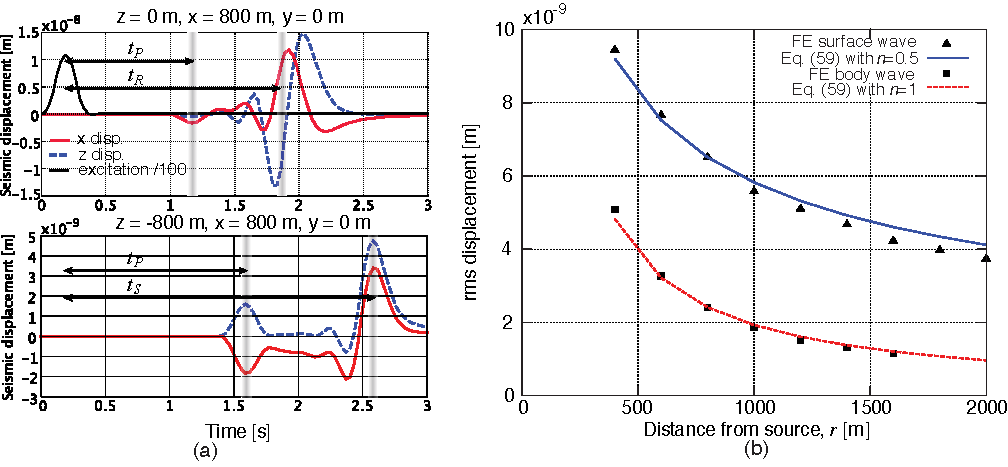
\includegraphics[width=0.9\textwidth]{./Sec_SiteInfra/Figures/Check_surfbulk.pdf} 
 		 \caption{(a) Finite element ground displacement measurements at a surface and subterranean location after a pulse excitation. P, S and Rayleigh wave arrival times are indicated. (b) The finite element results for the rms amplitude of the surface and body waves with increasing distance from the source. The geometric damping contribution to Eq.~(\ref{eq3.41}) is plotted for comparison.}
 	 	\label{CheckGGN}
 	 \end{center}
\end{figure}

As waves propagate through the medium, their amplitude decreases. This attenuation can be attributed to two factors; material and geometric damping. Geometrical damping is a result of energy spreading over an increasing area. The frequency dependent material damping involves energy lost due to friction. Seismic wave attenuation for homogeneous media, can be described by~\cite{seismic_kim}
\begin{equation}
	A_2 = A_1\left(\frac{r_1}{r_2}\right)^n e^{-\frac{\pi \eta f}{c}(r_2-r_1)},
	\label{eq3.41}
\end{equation}
where $A_1$ and $A_2$ denote the wave amplitudes at distance $r_1$ and $r_2$ from the source, $n$ represents the geometric damping coefficient, $f$ is  the frequency and $c$ the propagation speed of the wave. The material damping is represented by the loss factor $\eta$. The geometric damping coefficient can be determined analytically by assessing the type of wave involved and the source type. For radial surface waves $n=1/2$ while radial body waves within the medium decay with $n=1$.

To confirm the ground motion response calculated by a FE model, the arrival times and geometric damping of the wave fields can be studied. A homogenous half-space was simulated by creating a half-sphere model with no reflection of waves incident to the spherical boundary. In view of symmetry the model could be further simplified to a quarter half-space with symmetric boundary conditions on the vertical surfaces. A single vertical excitation force was applied uniformly within a circular area at the origin with a time dependent factor given by $F(t) = A \sin^2( \pi t/T_e)$ for $0\leq t \leq T_e$ where $T_e$ is the excitation period. The amplitude scaling factor, $A$, was adjusted to create a vertical displacement at the excitation point of 1 $\mu$m.

The model has parameters $E$ = 10 GPa, $\rho=2.0$ g/cm$^3$, $\nu=$ 0.25 and a radius of 2.2 km. This results in wave speeds of $c_P = 800$ m/s, $c_S = 462$ m/s and $c_R = 424$ m/s. No material damping was implemented in this model. 

Fig.~\ref{CheckGGN}a shows the FE results of seismic displacements along with expected arrival times at a location on the surface and at a depth of 800 m. Note the phase difference of $\pi/2$ between the $x$ and $z$ displacements of the Rayleigh wave. The rms wave amplitude with increasing distance from the source across the surface and within the medium are plotted in Fig.~\ref{CheckGGN}b. As expected from Eq.~(\ref{eq3.41}) the wave attenuation is proportional to $1/\sqrt{r}$ along the surface and $1/r$ within the medium. 
\begin{figure}[t] 
  	\begin{center}
   		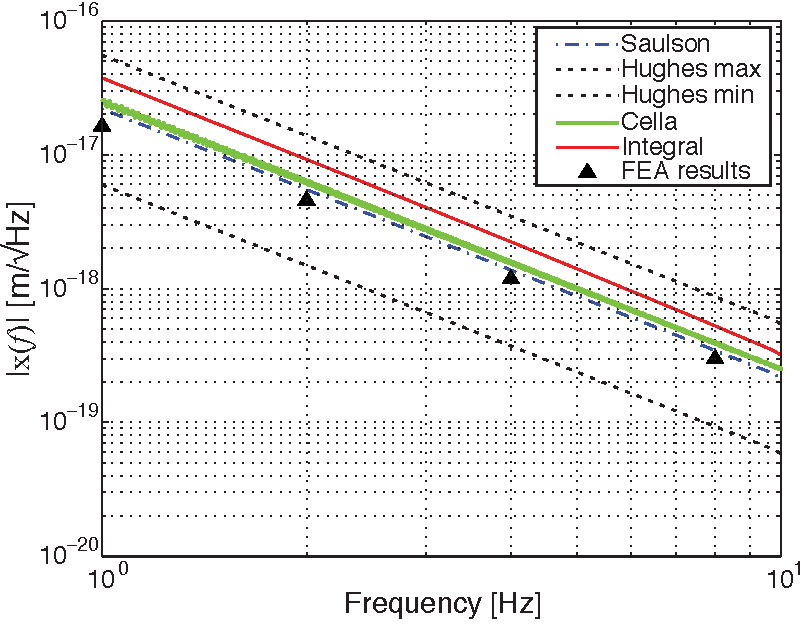
\includegraphics[width=0.49\textwidth]{./Sec_SiteInfra/Figures/ThorneSaulFEMcomparison_surface2.pdf} 
   		\caption{Finite element calculation of the Newtonian displacement noise amplitude for a surface detector. For comparison the results of Saulson, Cella, Hughes and Thorne, and the analytic integral are shown.}
   		\label{fig:FEresult}
   	\end{center}
\end{figure}

With the above model, we can calculate the NN for a given distribution of masses, which can be described by the mass density function $\rho(\mathbf{r},t)$. The resulting acceleration, experienced by a test mass (i.e.\ an interferometer mirror) located at $\mathbf{y}$, can be written as
\begin{equation}
	\mathbf{a}(\mathbf{y},t) = G \int_V \rho(\mathbf{r},t) \frac{\mathbf{r'}}{|\mathbf{r'}|^3}dV,
	\label{eq3.42}
\end{equation}
where $\mathbf{r}$ is the position of the mass volume $dV$ and $\mathbf{r'}=\mathbf{r}-\mathbf{y}$. In the FE analysis the acceleration is the summation of the contributions from each node $i$ with mass $m_i$ located at $\mathbf{r}_i$. The acceleration at the test mass is given by
\begin{equation}
	\mathbf{a} = \sum_i \mathbf{a}_i = \sum_i  G m_i \frac{\mathbf{r'}}{|\mathbf{r'}|^3},
	\label{eq3.43}
\end{equation}
with $G$ the universal gravitational constant. When a seismic disturbance is present, the nodes suffer a displacement denoted by $\mathbf{\xi}_i(\mathbf{r},t)$. The gravity gradient acceleration due to these displacements is given by
\begin{equation}
	\mathbf{a}^{NN}(\mathbf{y},t) = \sum_i (\nabla\otimes\mathbf{a}_i)^T \mathbf{\xi}_i(\mathbf{r},t).
	\label{eq3.44}
\end{equation}
Note that in the gravity gradient calculations presented here, the mass associated with each node is assumed to be constant. The corresponding analytical expression can be obtained by substituting $m_i \rightarrow \rho dV$ and evaluating the resulting integral.


The calculation of GGN via FE models was validated by creating simple rectangular homogenous half-space models, equivalent to those discussed by Saulson for a surface detector~\cite{GGSaulson}. The isotropic, elastic half-space with $\rho = 1.8$ g/cm$^3$, $\nu = 0.33$, $c_P = 440$ m/s and $c_S = 220$ m/s was excited on one boundary to yield plane harmonic pressure waves scaled to a flat ambient seismic noise spectrum of 1 nm/$\sqrt{\mbox{Hz}}$ between 1 and 10 Hz and the subsequent nodal displacements were recorded as a function of time. Boundary conditions were set such that no reflections occurred and seismic waves were continuous. The FE results are compared with the analytic results of Saulson and Hughes and Thorne~\cite{GGSaulson}\cite{GGThorne}. To facilitate comparison, an integral cut-off radius equal to that used in Saulson's analysis ($r_{\mbox{\scriptsize{cutoff}}} = \lambda/4$) was employed in the summation process. Fig.~\ref{fig:FEresult} shows that good agreement is obtained. To assess the effect of this cut-off the above model was calculated analytically using Eq.~(\ref{eq3.44}). Removing the cut-off leads to an increase of GGN by about a factor 2. The FE results approach those of the analytic expression in the limit that $r_{\mbox{\scriptsize{cutoff}}} $ decreases to zero. 
\begin{figure}[ht]
	\begin{center}
	\includegraphics[width=0.87\textwidth]{./Sec_SiteInfra/Figures/QS2Clay_paper.pdf}
	\caption{(a) Total displacement for a time domain simulation at 2.34 seconds after a 1 $\mu$m pulse excitation at the center of the half-sphere. (b) Time domain evolution of gravity gradient noise acceleration at a surface ($z$=0 m) and underground ($z$=-800 m) test mass. Only the horizontal component of the gravity gradient noise acceleration is shown. Arrival times of Rayleigh, S and P-waves are also indicated.}
		\label{fig:QS2Clay_paper}
	\end{center} 
\end{figure}

The pulse excitations and the half-sphere model described earlier, were used to investigate gravity gradients originating from nearby surface excitations (see Fig.~\ref{fig:QS2Clay_paper}). The nodal displacements were recorded as a function of time and the GGN was calculated at various depths on a vertical line at a distance $\lambda_P= 800$ m from the $z$-axis. In order to artificially separate the contributions of the surface and body waves to the GGN acceleration the nodes with a depth less than 200 m were summed separately from those deeper that 200 m. The respective surface and body contributions were combined to give a total acceleration. Note that for times shortly after the excitation, this distinction is not precise. The results for a test mass at the surface and a test mass at a depth of $\lambda_P$ are shown in Fig.~\ref{fig:QS2Clay_paper}. Only the GGN acceleration in the horizontal direction is shown since it has the largest effect on the performance of an interferometer. The expected arrival times of the different waves are indicated in the figures and show that the Rayleigh wave dominates the GGN contribution of a detector on the surface. At a depth of $\lambda_P$ the arrival of the S and P-waves can clearly be distinguished, the S-wave producing a larger contribution, attributed to the larger seismic displacements seen in Fig.~\ref{CheckGGN}a. The GGN contribution of a wave is initially negative as the wave approaches then changes sign as the wave passes by the test mass. It is interesting to note that the sign change of the surface contributions between a surface and underground detector. This is due to the sign change of the horizontal component of the Rayleigh wave for depths larger than 0.2$\lambda_R \approx 80$ m. The figure also shows that GGN builds up before any seismic disturbance actually reaches the test mass and for short times is only dependent on surface contributions.

\FloatBarrier
\subsubsection{Ambient NN subtraction}
\label{subsub:AmbientNNsubtraction}
A possible approach to the problem of NN mitigation is its subtraction. The
basic idea is to exploit the expected correlation between NN and a set of
auxiliary quantities which are continuously monitored \cite{CatichaPRE}. The
natural candidates for these are seismic displacement, and we can imagine a
basic scenario where a set of sensors (let's say displacement sensors) record
several time series. We will consider here the simplest scenario, namely we
suppose that the relevant quantities are stationary in a statistical
sense. The time series recorded by the I-th sensor will be $X_I = s_I
+ \sigma_I$, where $s_I$ is the seismic displacement evaluated at the sensor's
position and $\sigma_I$ its instrumental noise.

We will write the output of the interferometer as $Y = H + N$, where $N$ is
the $NN$ and $H$ the remaining part, which we suppose uncorrelated with the
seismic motion. The ``subtracted'' time series $Y_s$ has to be constructed in
such a way to satisfy a given optimization criterion. If each of the auxiliary
time series $X_I$ are uncorrelated with the gravitational wave's signal in $Y$
and the noise is Gaussian the optimal result can be obtained by
\begin{enumerate}
\item applying an appropriate linear and time invariant filter to each of the
$X_I$ signals
\item subtracting each filtered signal from $Y$
\end{enumerate}
The filters will be chosen in such a way to minimise the power spectrum of
$Y_s$, details are given in Box~\ref{box:optimalsubtraction}.

\longetbox{h}{box:optimalsubtraction}{Stationary noise: optimal subtraction}{
A simple way to state the problem is asking what is the linear combination of
the interferometer's and sensors' time series
\begin{equation}
	Y_{s}=Y(\omega)+\int d\omega '\sum_{I}\alpha_{I}(\omega,\omega ')X_{i}(\omega')
	\label{eq3.45}
\end{equation}
which we can call subtracted signal which minimise the power spectrum at each frequency. The minimisation variables are the functions $\alpha_{I}(\omega)$, which clearly represent linear filters that must be applied to the output of the sensors before adding them to the interferometer's data. The power spectrum $S_{Y_{s}Y_{s}}$ is related to the correlation by
\begin{eqnarray}
		\langle{Y_{s}(\omega)^{*}Y_{s}(\omega)}\rangle=\langle{Y(\omega)^{*}Y(\omega)}\rangle&+&\int d\omega '' \sum_{l}\alpha_{l}(\omega,\omega '')^{*}\langle{Y_{l}(\omega '')^{*}Y_{l}(\omega ')}\rangle\nonumber\\
		&+&\int d\omega ''d\omega ''' \sum_{I,J}\alpha_{I}(\omega,\omega '')^{*}\alpha_{J}(\omega ',\omega ''')\langle{Y_{I}(\omega '')^{*}Y_{J}(\omega ''')}\rangle\nonumber\\
		&+&\alpha_{l}(\omega ',\omega '')\langle{Y(\omega)^{*}Y_{l}(\omega '')}\rangle
		\label{eq3.46}
\end{eqnarray}
and minimizing this expression with respect to $\alpha_{K}(\omega ',\omega '')^{*}$ we obtain a set of linear integral equations for the optimal filters
\begin{eqnarray}
			\langle X_{K}(\omega '')^{*}Y(\omega ') \rangle+\sum_{J}\int d\omega ''\langle X_{K}(\omega '')^{*}X_{J}(\omega ''') \rangle\alpha_{J}(\omega ',\omega ''')=0
	\label{eq3.47}
\end{eqnarray}
In principle the expression of $\alpha_{J}$'s can be obtained by finding the inverse of the kernel $K_{KJ}(\omega,\omega')\equiv\langle X_{K}(\omega)^{*}X_{J}(\omega')\rangle$, formally
\begin{eqnarray}
		a_{I}(\omega',\omega)=-\sum_{K}\int d\omega'' K^{-1}_{IK}(\omega,\omega'')\langle X_{K}(\omega'')^{*}Y(\omega')\rangle
		\label{eq3.48}
\end{eqnarray}
If non stationary noise is present, we should define what is the relevant quantity that must be maximised, as the definition of the optimal apparatus sensitivity cannot be given it term of noise spectrum only. In the stationary case we can write
\begin{eqnarray}
		\langle X_{I}(\omega)^{*}Y(\omega')\rangle=2\pi\delta(\omega-\omega')C_{SN\,I}(\omega)
		\label{eq3.49}
\end{eqnarray}
Here the $I$, $J$ entry of the array $C_{SS}$ is the cross correlation between the seismic noise measured by the $I$th and $J$th sensors. Similar $C_{\Sigma\Sigma IJ}$ is the correlation between the intrinsic noises of the $I$th and $J$th sensors. Finally,
\begin{eqnarray}
		\langle Y(\omega)^{*}Y(\omega')\rangle=2\pi\delta(\omega-\omega')[C_{NN}(\omega)+C_{HH}(\omega)]
		\label{eq3.50}
\end{eqnarray}
is the decomposition of interferometer's power spectrum in a NN contribution plus all which is uncorrelated with it. Putting all this inside Eq.~(\ref{eq3.48}) and (\ref{eq3.46}) we get the optimal filters
\begin{eqnarray}
		\alpha_{I}(\omega,\omega')=-\delta(\omega-\omega')[C_{SS}(\omega)+C_{\Sigma\Sigma}(\omega)]^{-1}_{IJ}[C_{SN}(\omega)]_{J}
		\label{eq3.51}
\end{eqnarray}
which in the stationary case considered are time invariant, and the amplitude efficiency $\epsilon(\omega)$ of NN subtraction, which we define in terms of the ration between the power spectra of the subtracted $(S_{Y_{S}}(\omega))$ and un-subtracted $(S_{Y}(\omega))$ interferometer's signal spectral amplitude 
\begin{eqnarray}
		1-\epsilon(\omega)=\sqrt{\frac{S_{Y_{S}}(\omega)}{S_{Y}(\omega)}}=\sqrt{1-\frac{C^{+}_{SN}(\omega)[C_{SS}(\omega)+C_{\Sigma\Sigma(\omega)}]^{-1}C_{SN}(\omega)}{C_{nn}(\omega)}}
		\label{eq3.52}
\end{eqnarray}
Note that $(1-\epsilon)^{2}$ gives the ratio between the power spectra of the NN contained in the subtracted and un-subtracted signal. 
}

The ratio between subtracted and unsubtracted spectral noise amplitude, which is
given by Equation~(\ref{eq3.52}), is a function of 
\begin{itemize}
\item $C_{SS}$, an array whose entry in the $I$-th row and $J$-th column is
the spectral covariance between the $I$-th and the $J$-th sensor;
\item $C_{SN}$, a vector whose $I$-th entry is the spectral covariance between
the NN and the output of the $I$-th sensor;
\item $C_{NN}$, the power spectrum of NN.
\end{itemize}
This expression tell us that to achieve a good subtraction efficiency three
conditions are needed.
\begin{itemize}
\item All the sensors should be coupled as much as possible to NN, in other
words the correlation $C_{SN}$ between sensor's output and NN must be as large
as possible.
\item The intrinsic noise of the $I$-th sensor described by its power spectra
$[C_{SS}]_{II}$ should be small.
\item The correlation between quantities measured by different sensors,
described by $C_{SS}$, must also be small.
\end{itemize}

It is important to observe that when the procedure is correctly applied, it
will never reduce the sensitivity at each frequency.

Note that only the correlation among auxiliary sensors described by the
entries of the matrix $C_{SS}$ can be measured easily, so there is no real
hope to fully test the subtraction procedure without building a NN sensitive
detector. However Equation~(\ref{eq3.52}) can be estimated using a theoretical
model. We will use in the following the very simple one described in
Box~\ref{box:simplesubtractionmodel}. This is characterized by a single
(frequency dependent) correlation length $\xi(\omega)$.

\begin{figure}[t]
	\begin{center}
		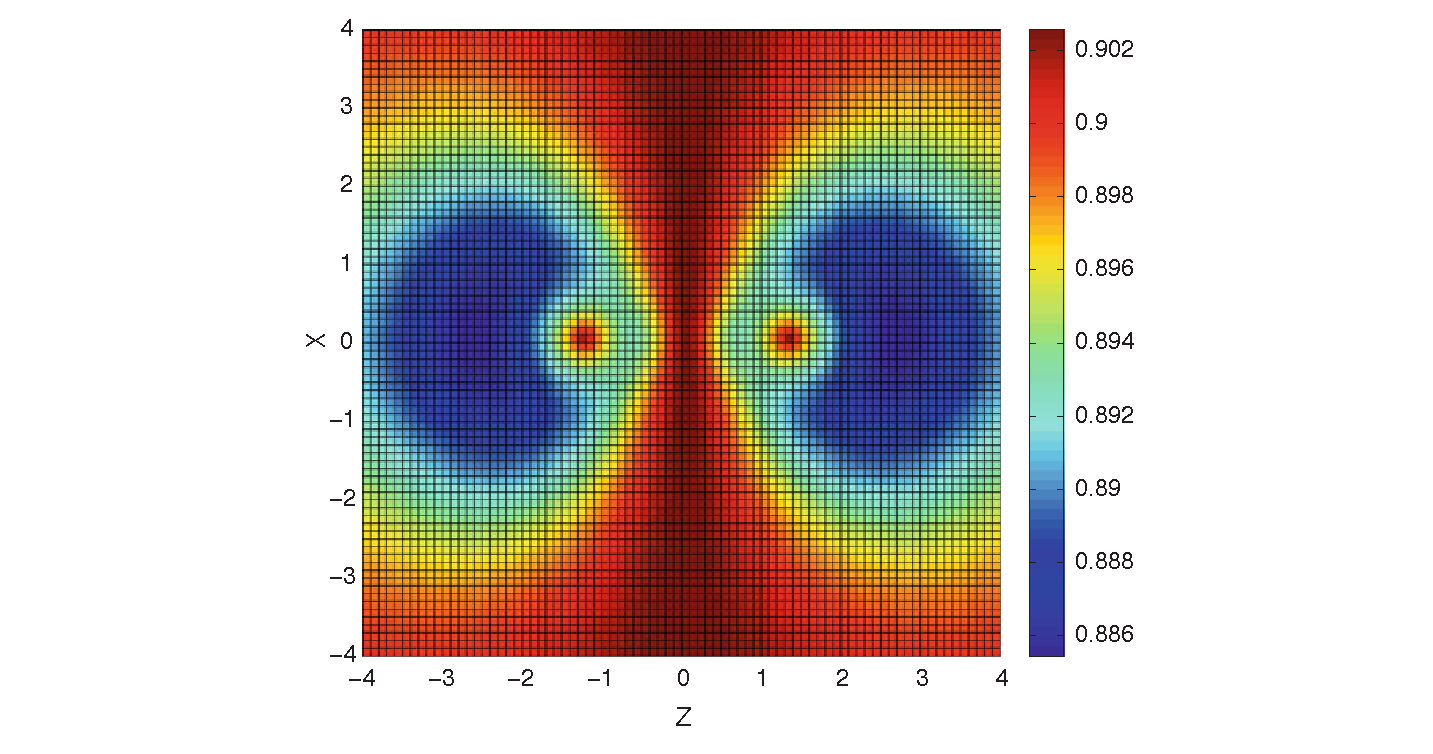
\includegraphics[width=16.5cm]{./Sec_SiteInfra/Figures/SimplOptSens.pdf}
		\end{center}
		\caption{The percentage reduction of NN on a single test mass with three sensors, for the model described by Eq.~(\ref{eq3.46}). The test mass is at the origin of the coordinate system, and the sensors measure the local density fluctuations. NN acceleration is sensed along the $z$ axis. Two sensors are fixed at their optimal positions, which are located at the circular spots at $(x,z)=(0,\pm)$. the quantity $1-\epsilon$ (see Eq.~(\ref{eq3.45})) is plotted as a function of the position of the third sensor. There is axial symmetry around the $z$ axis, so only the $x-z$ plane is displayed.}
\label{fig:NNreduction}
\end{figure}

\longetbox{h}{box:simplesubtractionmodel}{Simple subtraction model.}{
We consider a single test mass inside an infinite medium, and we suppose that each sensor can monitor the mass density fluctuation at its position. The $i$th sensor is also affected by a intrinsic noise $\sigma_{i}(f)$, without correlations between $\tilde{\sigma}_{i}$ and $\tilde{\sigma}_{j}$ when $i\neq j$. We model the density fluctuations as a Gaussian stochastic field described by an exponential cross correlation function
\begin{eqnarray}
		\langle\tilde{\rho}(\omega,{\bf x})^{*}\tilde{\rho}(\omega',{\bf x}')^{*}\rangle=2\pi\Gamma(\omega)^{2}\delta(\omega-\omega')\exp\Big{(}-\frac{|{\bf x}-{\bf x'}|}{\xi(\omega)}\Big{)}
		\label{eq3.53}
\end{eqnarray}
The correlation functions relevant for the subtraction are easily evaluated, obtaining
\begin{eqnarray}
		C_{SS}(\omega)_{IJ}+C_{\Sigma\Sigma}(\omega)_{IJ}&=&\Gamma(\omega)^{2}\exp(-|{\bf u}_{i}-{\bf u}_{j}|)+\sigma^{2}(\omega)\delta_{IJ}\\
		C_{SN}(\omega)_{I}&=&4\pi\xi G\Gamma(\omega)^{2}\cos\theta_{I}\Psi(u_{I})\\
		C_{NN}(\omega)&=&\frac{16}{3}\pi^{2}\xi^{2}G^{2}\Gamma(\omega)^{2}
		\label{eq3.54}
\end{eqnarray}
where ${\bf u}_{I}=\xi^{-1}{\bf r}_{i}$ is the position of the $I$-th sensor measured in $\xi$ units, $\theta_{I}$ the angle between the axis along which the Newtonian acceleration is measured and the sensor's position vector and
\begin{eqnarray}
		\Phi(u)=\frac{1}{u^{2}}\Big{[}2-e^{-u}\Big{(}2+2u+u^{2}\Big{)}\Big{]}
		\label{eq3.55}
\end{eqnarray}
For a given arrangement of the sensors Eq.~(\ref{eq3.52}) becomes
\begin{eqnarray}
		1-\epsilon=\sqrt{1-3\Big{(}e^{-|{\bf u}_{I}-{\bf u}_{J}|}+\frac{\sigma^{2}}{\Gamma^{2}}\delta_{IJ}\Big{)}^{-1}\Phi(u_{I})\Phi(u_{J})\cos\theta_{I}\cos\theta_{J}}
		\label{eq3.56}
\end{eqnarray}		
}


One issue to be investigated is connected with the optimal way in which the
set of sensors available must be displaced on the field, by optimizing
Eq.~(\ref{eq3.56}) over the positions and the orientations.

With two sensors only the optimal positions are on the Newtonian acceleration axis, at a distance $d\simeq \pm 1.281 \xi$ from the est mass (we will consider only the $\sigma=0$ case). The $\cos\theta$ factor is maximised along the axis, while $\Phi(u)$ has a maximum at $u\simeq1.451$. In this optimal case $1-\epsilon\simeq0.902$. If we add a third sensor, we can evaluate $1-\sigma$ as a function of its position, which the other two fixed. This is represented in figure~\ref{fig:NNreduction}, assuming that the NN is measured along the $z$ axis. We can see how the subtraction efficiency changes with the position of the sensor, measured in unit of the correlation length. There is no improvement if we put the third sensor near the others, due to the complete correlation of the new measurement with the others. We do not gain anything from far from the test mass or at $z=0$, because in this case the measure is uncorrelated to NN. the best positions are along the $z$ axis, at a distance roughly doubled from the center. 

The model is quite crude so these are only indicative results. However, the model does show one particular feature. The separation between the sensors must be optimized accordingly with the typical correlation length $\xi$ of the contributions to NN we want to subtract, which depends on the frequency band where the subtraction is needed. 	
\begin{figure}[t!]
	\begin{center}
		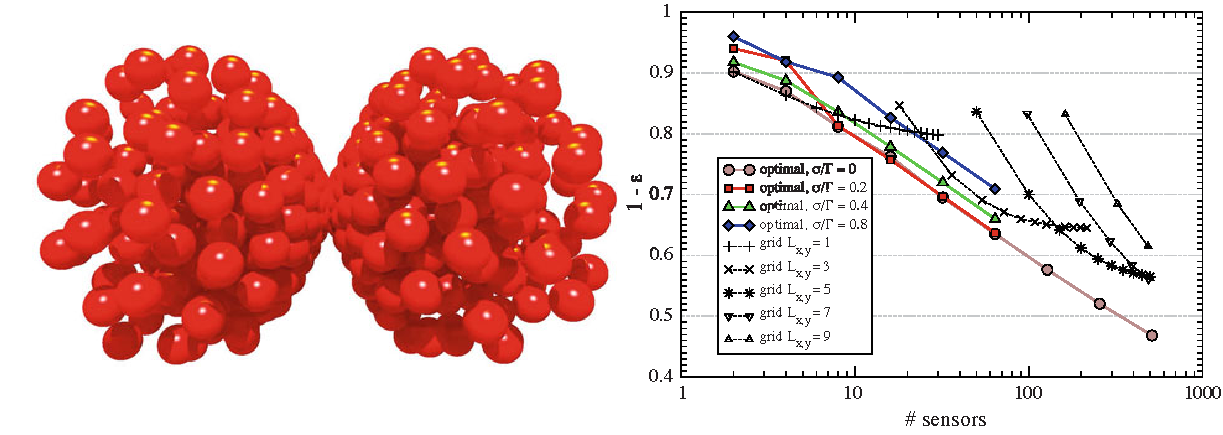
\includegraphics[width=16.5cm]{./Sec_SiteInfra/Figures/SimplOptSens2.pdf}
		\end{center}
		\caption{Left). The optimal positions for 512 sensors, evaluated accordingly with the model~(\ref{eq3.46}). Each sensor is supposed to measure the local fluctuation of density, and is represented as a sphere with the center on its position and radius $\xi$. The single test mass considered is at the centre of the two clouds, and the NN is measured along the approximate axis of symmetry of the distribution. Right). The percentage of NN on a single test mass as a function of the number of auxiliary sensors, accordingly with the model~(\ref{eq3.46}). The sensors are supposed to measure the local fluctuation of density. Solid lines correspond to optimal configurations, evaluated for different intrinsic noises of the sensors. Dashed curves correspond to regular grids with sizes $L_{x}=L_{y}$ and $L_{z}$. The grid is centred on the grid and the number of sensors given by $L_{x},L_{y},L_{z}$. The NN is sensed along the $z$ axis, and $\sigma=0$ in this case.}
\label{fig:OptimalPosition}
\end{figure}

Another important point to understand is how the subtraction procedure improves with the number of sensors, and how much it is sensitive to a non optimal placement of the sensors. This is important because in a practical implementation the possibility of optimizing the placement will be limited, especially if the number of sensors will be large. It must be remembered that the optimization of the sensors' positions is a global process and all the parameters must be changed at the same time. 

Remaining in the framework of the simple model considered we optimized Eq.~(\ref{eq3.56}) for a different number of sensors. We used a simulated annealing procedure to be reasonably sure to find a global minimum. A typical result for the optimal configuration of the sensors is shown in the left illustration of Fig.~\ref{fig:OptimalPosition}. We considered 512 sensors, adjusting their positions. Each sphere in the plot has a radius length $\xi$, and is centered on a sensor's position. We see that the spheres attempt to cover the region which is maximally coupled to NN acceleration (the test mass is between the two clouds), but they attempt also not to overlap in order to minimise the correlation between sensors. Fig. 8 correspond to the optimal configuration in the $\sigma= 0$ case. We do not show similar plots for $\sigma > 0$, however in that case we found that the overlap between the spheres increases with $\sigma/\Gamma$. This is expected because in that case a correlation between detectors can be compensated by the average of intrinsic noises. 

In the right plot of Fig.~\ref{fig:OptimalPosition} we show the relative reduction of NN as a function of the number $N$ of auxiliary sensors. The reference plot is labeled with circles, and it corresponds to the optimal configuration in the $\sigma= 0$ case. We see that the reduction of NN is quite modest, and improves slowly with N. This is partly due to the chosen model, which is quite bad from this point of view, a scan be seen with the following argument. Each sensor can be used at best to subtract the contribution to the NN of a sphere of radius $\xi$ centered on it. The number of non overlapping spheres at distance $\xi$ from the test mass scales as $n^2$, while the contribution of each of them to NN scales as $n^{-2}$. We have to sum all the contributions in quadrature, so if all the spheres with $n<N$ are monitored we expect for large $n$ that $1-\epsilon\sim\sqrt{\sum^{\infty}_{k}k^{-2}}\sim n^{-1/2}$ or as the number of sensors $N_{s}$ scales as $n^{3}$, $1-\epsilon\sim N^{-1/6}_{s}$. 

Different models are expected to allow better subtraction performances, especially when the loss of coherence described by the scale $\xi$ is less relevant. This could be the case in some geological scenarios, while in others the simplified model presented can give an adequate description. It is an important issue, which is currently under careful investigation. 
\begin{figure}[t!]
	\begin{center}
		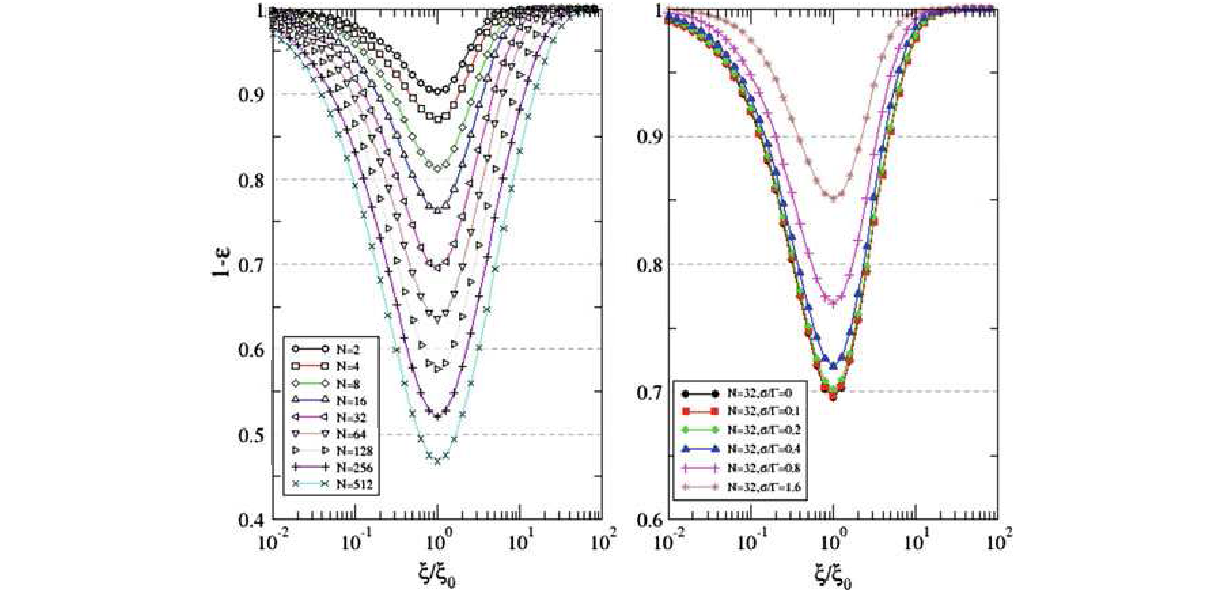
\includegraphics[width=16.5cm]{./Sec_SiteInfra/Figures/SimplOptSens3.pdf}
		\caption{On the left, the reduction of NN for a configuration of the sensors optimized for $\xi=\xi_{0}$, as a function of the ratio $\xi(\omega)/\xi_{0}$, where $\xi(\omega)$ correspond to the observed frequency. The different plots correspond to different number of sensors. On the right, for $N=$32 sensors in the configuration optimized at $\xi=\xi_{0}$, the reduction of NN is plotted as a function of $\xi(\omega)/\xi_{0}$. The different plots correspond to different values of the intrinsic noise of the sensors.}
		\label{fig:OptimalRedution}
	\end{center}
\end{figure}

Coming back to the right plot in Fig.~(\ref{fig:OptimalPosition}), the plots labeled with squares, triangles and diamonds gives $1-\epsilon$ for the optimal configuration in presence of some amount of instrumental noise. As expected there is a reduction of the subtraction performances. Finally, we showed in the same figure for comparison the results which can be obtained with a non optimal configuration, namely a regular grid of detectors with different sizes $L_x = L_x$ and $L_z$ , centered on the test mass. The optimization here is done only on the grid size, and $\sigma = 0$. The best regular grids correspond to the shapes which are best overlapped to the region coupled to NN, which means $L_{z} > 2L_{x, y}$. 

The optimization of the positions of sensors can clearly be done at a given coherence length $\xi(\omega)$, while the subtraction procedure will be applied to an entire range of frequencies (we can assume for definiteness $\xi$ proportional to the frequency). This means that the subtraction will be optimal at a chosen frequency only. 

In Fig.~\ref{fig:OptimalRedution} (left) we plotted the NN reduction as a function of the ratio $\xi(\omega)/\xi_{0}$ between the coherence length at the observed frequency and the one $\xi_{0}$ which correspond to the optimized sensors' configuration. Different plot correspond to a different number of sensors, and $\sigma=0$. A sensible reduction of the subtraction performance is evident when $\xi$ changes by one order of magnitude. This reduction is somewhat decreased by a large number of sensors. 

The effect of noise can be seen in Fig.~\ref{fig:OptimalRedution} (right). Here the number of sensors is fixed at 32, and different plots correspond to different values of $\sigma/\Gamma$. The plot suggest (with some extrapolation) that to achieve an hundred fold NN suppression, rock density (and position) fluctuations need to be measured in real time with resolution less than 1\% of the actual motion (in quiescent times in a quiet location), i.e.\ $\sigma/\Gamma < 10^{-2}$ . Because the available seismometers have been mainly developed to detect seismic events, their sensitivity is just below the normal rock activity level. A well defined subtraction pipeline has to be tested with models in order to give a precise estimate, however our conservative expectation is that seismic sensors 100 times more sensitive than currently employed must be developed for NN suppression to become useful. Preliminary studies in this direction are being done at Homestake, specifically in the direction of laser strain meters and high sensitivity dilatometers. We expect that these developments, if successful, will also yield important side results in geology.

\FloatBarrier
\subsubsection{NN subtraction from periodic sources}
\label{subsub:NNsubtractionperiodic}
Active NN subtraction schemes have been studied both at the LIGO and Virgo laboratories \cite{Beker2010GRG, Pepper2007, Harms22009}. Methods for active NN subtraction involve placing a witness sensor (seismometer) that monitors the noise source and estimates the noise transfer function by methods of minimising a cost function $J$ (difference between the measured noise and the estimated transfer function times the seismometer signal). The cost function that is commonly used in filter design optimisation, is the mean-square error (MSE). Minimising the MSE involves only second order statistics (correlations) and stems from the theory of linear filtering, which has many practical applications. In general, the idea is to recover a desired signal $d(n)$ given a noise observation $x(n)=d(n)+v(n)$ by using some linear filter with coefficients ${\bf w}$. Minimising the cost function 
\begin{eqnarray}
		J=  E\{e^{2}(n)\} = E\{ (d(n)-\hat{d}(n))^{2}\} = E\{ (d(n)- {\bf w}^{T}{\bf x}(n))^{2}\} 
\end{eqnarray}
with the provisions that the derivative of $J$ with respect to ${\bf w}$ and the second derivative to ${\bf w}$ are zero and positive respectively, provides the Wiener, or optimal filter solution, which is useful for filter coefficients that are constant in time. If we assume that the seismic spatial distribution, generated by pumps and electricity generators, can be approximated by a Gaussian distributed impulse acting vertically onto the soil, we can use the finite element results to attempt to estimate and subtract the NN from our gravitational wave data channels. 
\begin{figure}[h!]
	\begin{center}
		\includegraphics[width=16.5cm]{./Sec_SiteInfra/Figures/nngeneration.pdf}
		\caption{Results of time domain finite element simulations for NN. The grey bars indicate the arrival times and contributions from the pressure and shear wave components. Top left) Element displacement after a 1 $\mu$m pulse excitation at the center of the half-sphere. Bottom left). Element displacement at an underground location ($x$=800 m, $z$=-800 m) after pulse excitation at the centre of the half-sphere. Top right). Newtonian acceleration at the surface of the half sphere due to a pulse excitation. Bottom right). Newtonian acceleration at an underground location ($x$=800 m, $z$=-800 m) due to a pulse excitation.}
		\label{fig:NNfigure1}
	\end{center}
\end{figure}

Figure~\ref{fig:NNfigure1} is a combination of two previous plots (Fig. \ref{CheckGGN}a and Fig. \ref{fig:QS2Clay_paper}b) and shows the FE results of a typical time domain soil displacements and NN response as a function of time. The top and bottom plots on the left show the seismic excitation and the resulting displacement amplitudes at the centre of the homogeneous half space and at a depth of 800m respectively. The top and bottom plots on the right of Fig.~\ref{fig:NNfigure1} show the resulting Newtonian acceleration for a test mass placed on the surface of the half space, 800m from the excitation point and the Newtonian acceleration for a test mass placed at a distance of $\sim$1130m and a depth of 800m below the surface. Note that, in both cases, as soon as the excitation occurs a Newtonian acceleration is present at the test mass. 

The left and right plots in Fig.~\ref{fig:NNfigure1} can be interpreted as individually measured quantities, i.e.\ a NN signal in our GW detector (right) and a seismic disturbance that is measured at it's source (left). Since the disturbance is impulse like, we can estimate the NN impulse response due this disturbance from this specific source. 

After ET becomes operational, it will be of great importance to minimise localised anthropogenically generated seismicity. This does not stop at restricting access to areas close to the interferometer test masses. Thorne \emph{et al.} investigated how the interferometer is affected by NN originating from humans, animals, airplanes, etc.~\cite{GGthorneWinstein}. Within the subterranean environment this extends to placement of electricity generators, pumps, and cryo-coolers to keep the facility operational. These devices will be sources of seismic noise and will therefore generate continuous NN. 

%Figure~\ref{fig:NNfigure2} shows the time domain estimation and subtraction results obtained using the data displayed in Fig.~\ref{fig:NNfigure1}. After the initial Wiener coefficients have been obtained, a periodic signal is placed at the center of the half sphere. Using the knowledge of the noise transfer function we can estimate the NN due to the excitation close to the seismic sensor. As can be seen, typical estimates allow subtractions of at least an order of magnitude.   
%\begin{figure}[t!]
%	\begin{center}
%		\includegraphics[width=16.5cm]{./Sec_SiteInfra/Figures/nnsubtraction.pdf}
%		\caption{Subtraction of NN originating from a pump using a single seismometer and a Wiener filter.}
%		\label{fig:NNfigure2}
%	\end{center}
%\end{figure}




